\documentclass{article}



\usepackage{arxiv}

\usepackage[utf8]{inputenc} % allow utf-8 input
\usepackage[T1]{fontenc}    % use 8-bit T1 fonts
\usepackage{hyperref}       % hyperlinks
\usepackage{url}            % simple URL typesetting
\usepackage{booktabs}       % professional-quality tables
\usepackage{amsfonts}       % blackboard math symbols
\usepackage{nicefrac}       % compact symbols for 1/2, etc.
\usepackage{microtype}      % microtypography
\usepackage{lipsum}		% Can be removed after putting your text content
\usepackage{graphicx}
\usepackage{natbib}
\usepackage{doi}
\usepackage{subcaption}



\title{Architectural Style Classification}

%\date{September 9, 1985}	% Here you can change the date presented in the paper titlehttps://www.overleaf.com/project/65695666e775b7281d7f6e99
%\date{} 					% Or removing it

\author{
    {\hspace{1mm}Cheng Fei} \\
	Cornell Tech\\
	New York, NY \\
	\texttt{cf482@cornell.edu} \\
    \And
    {\hspace{1mm}Tianyu Lou} \\
	Cornell Tech\\
	New York, NY \\
	\texttt{tl838@cornell.edu} \\
	%% examples of more authors
	\And
	{\hspace{1mm}Wenjie Wang} \\
	Cornell Tech\\
	New York, NY \\
	\texttt{ww523@cornell.edu} \\
	%% \AND
	%% Coauthor \\
	%% Affiliation \\
	%% Address \\
	%% \texttt{email} \\
	%% \And
	%% Coauthor \\
	%% Affiliation \\
	%% Address \\
	%% \texttt{email} \\
	%% \And
	%% Coauthor \\
	%% Affiliation \\
	%% Address \\
	%% \texttt{email} \\
}

% Uncomment to remove the date
%\date{}

% Uncomment to override  the `A preprint' in the header
%\renewcommand{\headeright}{Technical Report}
%\renewcommand{\undertitle}{Technical Report}
%\renewcommand{\shorttitle}{\textit{arXiv} Template}

%%% Add PDF metadata to help others organize their library
%%% Once the PDF is generated, you can check the metadata with
%%% $ pdfinfo template.pdf
\hypersetup{
pdftitle={A template for the arxiv style},
pdfsubject={q-bio.NC, q-bio.QM},
pdfauthor={Tianyu Lou, Wenjie Wang, Fei Cheng},
pdfkeywords={First keyword, Second keyword, More},
}

\begin{document}
\maketitle

\begin{abstract}
    This research paper introduces a novel architecture style classification model aimed at discerning various architectural styles based on their visual characteristics. As individuals explore new environments, encountering buildings of historical or unique significance often sparks curiosity about their architectural styles and the narratives they encapsulate. However, recognizing and cataloging diverse architectural styles can be challenging for humans due to their sheer abundance and complexity. In response to this challenge, our study proposes the development of an architecture style classification model capable of real-time recognition. This model holds promising applications, particularly for tourists who can capture images of buildings and promptly identify their architectural styles. The primary objective is to create a system adept at recognizing architectural styles across different historical eras and various architects' designs. By employing advanced visual recognition techniques, our model aims to contribute to the seamless integration of technology into architectural appreciation, providing an accessible tool for enthusiasts, historians, and tourists alike. The potential impact of such a model extends beyond individual curiosity, offering a practical solution for instant architectural style identification in diverse scenarios.
\end{abstract}


% keywords can be removed
\keywords{Architectural Style \and Convolutional Neural Network \and ResNet}


\section{Introduction}
The rich tapestry of architectural styles that grace our cities and landscapes stands as a testament to the diverse creativity of human civilization. However, for individuals navigating urban environments or exploring historical sites, the challenge of identifying and understanding the architectural styles of buildings remains a significant barrier to a deeper appreciation of our built heritage. This paper introduces ArchVisioNet, an innovative architecture style classification model designed to address this challenge by leveraging advanced visual recognition techniques. As technology continues to intersect with various facets of our lives, the fusion of artificial intelligence and architectural appreciation takes center stage in ArchVisioNet. This model not only aims to unravel the complexities of architectural styles in real-time but also seeks to empower users, especially tourists, enthusiasts, and historians, with a tool capable of providing instantaneous insights into the historical eras and architects behind diverse architectural designs. Through a synthesis of cutting-edge technology and a passion for architectural heritage, ArchVisioNet represents a pioneering step towards democratizing architectural knowledge and fostering a deeper connection between individuals and the rich architectural tapestry that surrounds them.


\section{Background}
% \label{sec:headings}
%  \ref{sec:headings}.
\subsection{Context}
In comparing our project on architectural style classification using Convolutional Neural Networks (CNN) with significant prior works in the field, we observe both continuities and advancements. Our project draws inspiration from Alex Krizhevsky, Ilya Sutskever, and Geoffrey E. Hinton's groundbreaking work on ImageNet Classification with Deep Convolutional Neural Networks, which revolutionized the approach to deep learning in image classification. While their work laid the foundation for using deep CNNs, our project extends these principles specifically to architectural styles, emphasizing the nuanced differences and unique characteristics inherent in this type of imagery.

Similarly, the work of Kaiming He and his colleagues on Deep Residual Learning for Image Recognition, particularly their development of ResNet, influenced our model's architecture. The deep residual learning framework they introduced allowed us to build deeper networks, crucial for capturing the intricate details necessary in architectural classification. However, our project diverges in its application and fine-tuning, tailoring the model to recognize and differentiate between architectural styles rather than the broader object recognition in He et al.'s study.

Furthermore, our project benefits from advances in transfer learning and data augmentation, concepts not fully explored in these earlier works. We leverage pre-trained networks and sophisticated data augmentation techniques to address the unique challenges of architectural image classification, such as varied lighting conditions and perspectives. These advancements demonstrate our project's evolution beyond the foundational work, focusing on specialized applications of CNNs in a domain-specific context.

\subsection{Architectural Styles}
Architectural styles refer to the distinct characteristics and features that define the appearance and structure of buildings across different periods and regions. These styles are categorized based on elements like form, method of construction, building materials, and regional cultural influences. Common examples include Gothic, Romanesque, Baroque, Victorian, Modernist, and Postmodernist styles. The classification of architectural styles is crucial in the fields of art history, urban planning, and conservation, aiding in the understanding of cultural and historical contexts of architecture.

\subsection{Dataset}
The initial dataset consists of 25 distinct architectural styles, each represented by 400 images on average. We generate the dataset from the ground up by extracting images from online sources like Google Images and assigning each image a corresponding label manually. In order to increase the quality of scraped datasets, we optimize the python crawler to filter out noisy datasets. Generally, these architectural styles are among the most common ones people can find in their daily lives, which ensures the applicability and feasibility of the model.

Subsequently, we undertake data preprocessing tasks, ensuring that all images are standardized in size without sacrificing any key features, and noisy information is removed which consists of reorientation and rescaling. Then, we perform data augmentation to produce a large batch of data in order to optimize the model accuracy. This step consists of adjusting the sharpness, color, brightness, and contrast.

\begin{figure}[h]
    \centering

    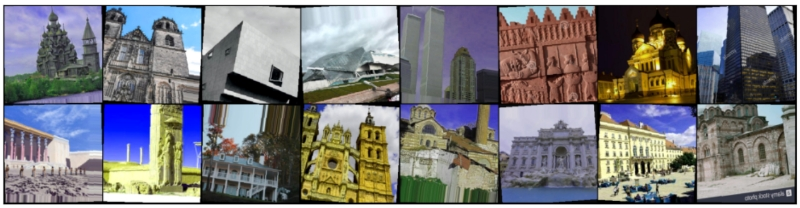
\includegraphics[width=0.5\linewidth]{images/Data_Visual.jpg}   
    \caption{Dataset Visualization}
    \label{fig:train_acc}
\end{figure}

\subsection{Convolutional Neural Network}
CNNs are a class of deep neural networks, primarily used in processing data with a grid-like topology, such as images. They are exceptionally adept at recognizing patterns in images, making them ideal for tasks like image classification, object detection, and even style transfer. A CNN automatically detects important features without any human supervision, using a series of convolutional and pooling layers. Each layer in a CNN transforms the input data to enable the network to learn more complex features in deeper layers, making it a powerful tool for image analysis.

\subsection{Transfer Learning}
Transfer learning is a machine learning technique where a model developed for one task is reused as the starting point for a model on a second task. In the context of CNNs, this often means using a pre-trained network that has already learned a comprehensive set of image features on a large dataset (like ImageNet). The pre-trained network can then be fine-tuned with a smaller dataset specific to the target task, such as architectural style classification. This approach is beneficial because it significantly reduces the computational resources and time required to train a deep neural network, while often enhancing performance, especially when the available dataset for the new task is relatively small.

This model leverages the pattern recognition power of CNNs and the efficiency of transfer learning. It can identify and classify various architectural styles from images, which can be an invaluable tool in fields like cultural heritage conservation, urban development, and even education in architectural history.

%\subsubsection{Headings: third level}


\section{Method}
% \label{sec:others}
\subsection{Data Preprocessing}
Data preprocessing prepares the dataset for the training task. We perform two major steps in order to expedite the training procedures.

\emph{\textbf{Normalization:}} For image data, normalization usually involves adjusting the pixel values. Since pixel values range from 0 to 255, a common practice is to scale these values to a range of 0 to 1. This is done by dividing all pixel values by 255. This scaling helps in speeding up the convergence by reducing the variability in the input data. Normalization helps in optimizing the training speed by making the training process more stable and efficient, and by preventing issues like vanishing or exploding gradients in deep learning models.

\emph{\textbf{Auto-tuning:}} In distributed training scenarios, auto-tuning can optimize the allocation of computational resources (like CPUs and GPUs) to different parts of the model or data, ensuring that the training process is as fast as possible. Auto-tuning is particularly beneficial in reducing the manual effort involved in hyper-parameter tuning and in achieving faster convergence with optimal resource utilization. It helps in ensuring that the model trains efficiently without the need for extensive manual experimentation.

\subsection{Data Augmentation}
Data augmentation is a crucial step in improving the performance and robustness of machine learning models, particularly in image classification tasks like Architectural Style Classification. Here are some data augmentation techniques we used in the model:

\emph{\textbf{Rotation:}} This is especially useful as buildings and architectural photographs can be captured from different angles.\\
\emph{\textbf{Flipping}}: This can be particularly useful for symmetrical structures.\\
\emph{\textbf{Scaling}}: This is important because architectural photos can be taken from various distances, altering the apparent size of the structure in the image.\\
\emph{\textbf{Cropping}}: Random cropping of images can simulate partial views of buildings, a common scenario in architectural photography, especially in urban settings where full views are often obstructed.

\emph{\textbf{Brightness Adjustment}}: Architectural photos can be taken in various lighting conditions, from bright sunlight to overcast skies.\\
\emph{\textbf{Contrast Adjustment}}: This trains the model to be more adaptable to variations in image quality and style representation.\\
\emph{\textbf{Color Adjustment}}: Adjusting the color properties of the images (like saturation, hue, etc.) can help the model in recognizing styles under different color conditions and photographic styles.\\
\emph{\textbf{Perspective Adjustment}}: This helps the model understand architectural styles in a three-dimensional context.

\emph{\textbf{Adding Noise}}: Introducing a small amount of random noise (like Gaussian noise) can improve the robustness of the model against grainy or low-quality images.\\
\emph{\textbf{Adding Filter}}: Using various filters (like edge enhancement, sharpening, etc.) can help in highlighting or suppressing specific features of architectural designs, aiding in better feature extraction by the CNN.

\subsection{Integration of Residual Networks in CNN}
\emph{\textbf{Skip Connections:}} The core idea behind ResNet is these skip connections that allow the input to “skip over” some layers. These connections simply perform identity mapping, and their outputs are added to the outputs of the stacked layers. Technically, they bypass or 'skip' one or more layers and connect to a later layer in the network. This approach allows the model to carry forward features from previous layers without the risk of degradation during deeper layers.

\emph{\textbf{Applications:}} In our project, we utilize ResNet due to its ability to efficiently train deeper networks, a necessary requirement for the complex task of architectural style classification. The intricate details and subtle nuances of architectural styles demand a network capable of extracting deep, sophisticated patterns. ResNet, with its deep structure enhanced by skip connections, ensures that our model learns these intricate patterns without suffering from the vanishing gradient problem, thus leading to more accurate and reliable classifications.

\section{Setup}

The development of the CNN model goes through four major stages: model selection, initial model construction, parameter fine-tuning, and performance evaluation.

\subsection{Phase 1: Model Selection}

\begin{figure}[h]
    \centering
    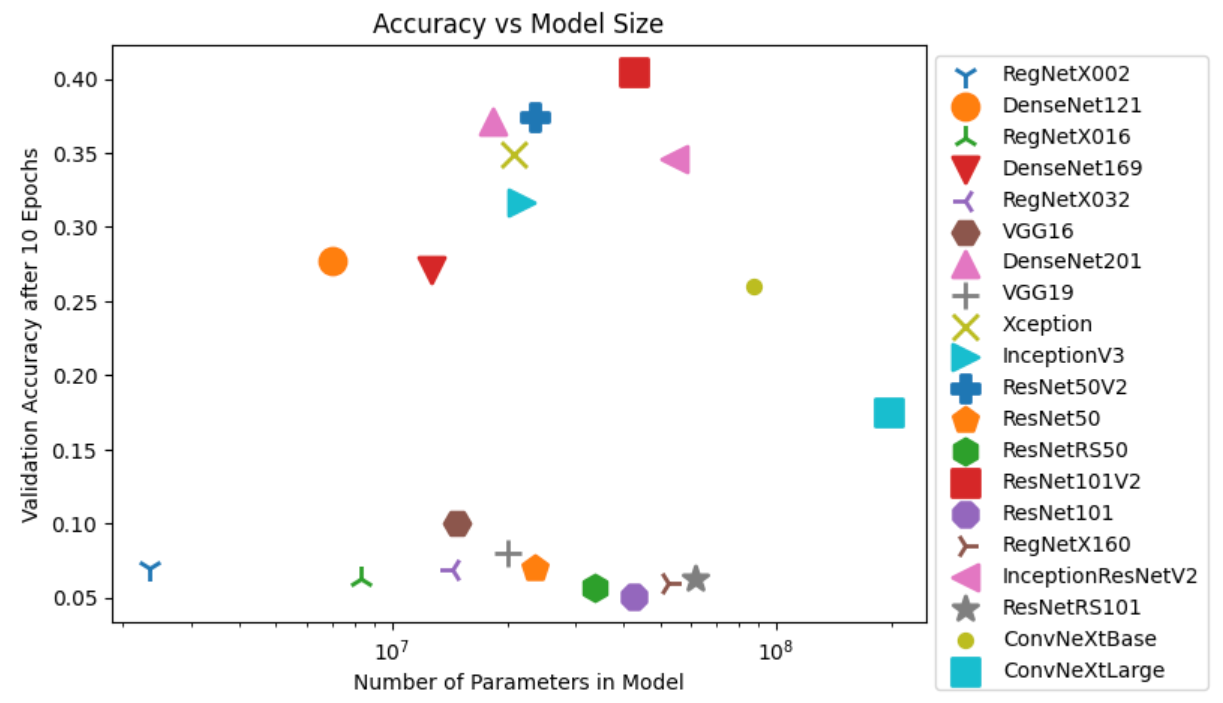
\includegraphics[width=0.5\linewidth]{images/model_selection.jpg}
    \caption{Different Model Accuracy}
    \label{fig:mono}
\end{figure}
To identify the most suitable CNN architecture for classifying architectural images, we conducted a thorough evaluation of various Convolutional Neural Network (CNN) architectures to determine the most suitable model for classifying architectural images in our initial phase of research. This evaluation encompassed a diverse range of CNN models, including well-known architectures such as VGG, Inception, and ResNet. Each of these models was assessed for their potential effectiveness in our specific application. Ultimately, the ResNet architecture was selected for its advanced residual learning framework. This framework is particularly beneficial as it effectively combats the vanishing gradient problem that often plagues deep neural networks, ensuring consistent learning even as the network depth increases. The selection criteria were not solely based on architectural features; we also considered critical performance metrics. These included the accuracy of the model and the speed of convergence during preliminary testing. Another key factor in our decision was the model's ability to handle deep architectures without significant performance degradation. ResNet's capability to maintain robust performance in deep network structures, without losing efficiency or accuracy, made it the standout choice for our complex image classification task.

\subsection{Phase 2: Initial Model Development and Overfitting Challenges}
\begin{figure}[h]
    \centering

    \begin{subfigure}{0.5\linewidth}
        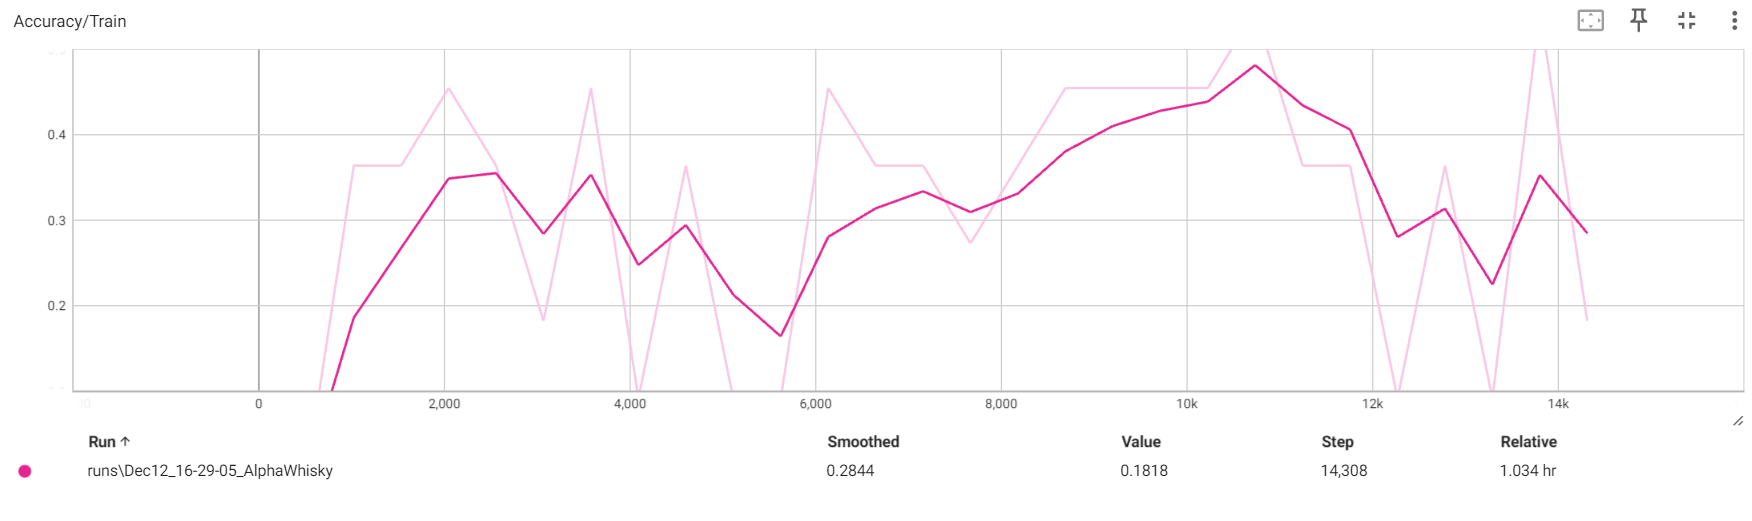
\includegraphics[width=\linewidth]{images/ResNet5_train_acc.jpg}   
        \caption{ResNet5 Training Accuracy}
        \label{fig:train_acc}
    \end{subfigure}%
    \begin{subfigure}{0.5\linewidth}
        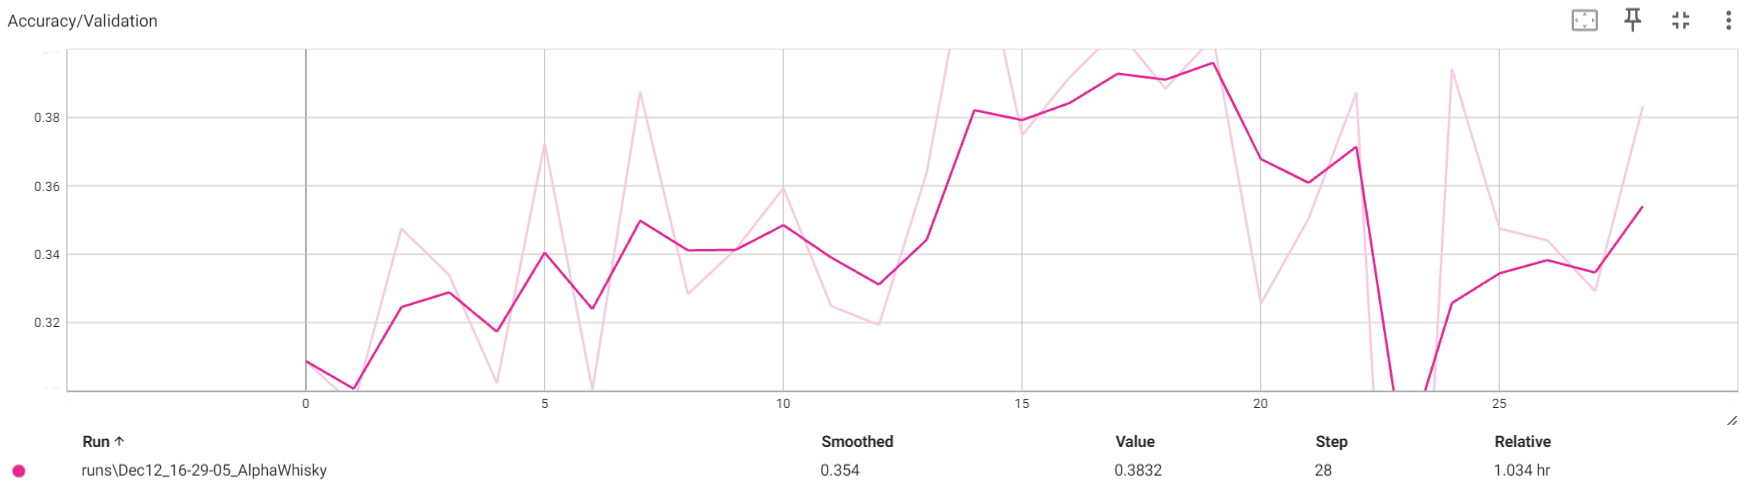
\includegraphics[width=\linewidth]{images/ResNet5_val_acc.jpg}
        \caption{ResNet5 Validation Accuracy}
        \label{fig:val_acc}
    \end{subfigure}

    \begin{subfigure}{0.5\linewidth}
        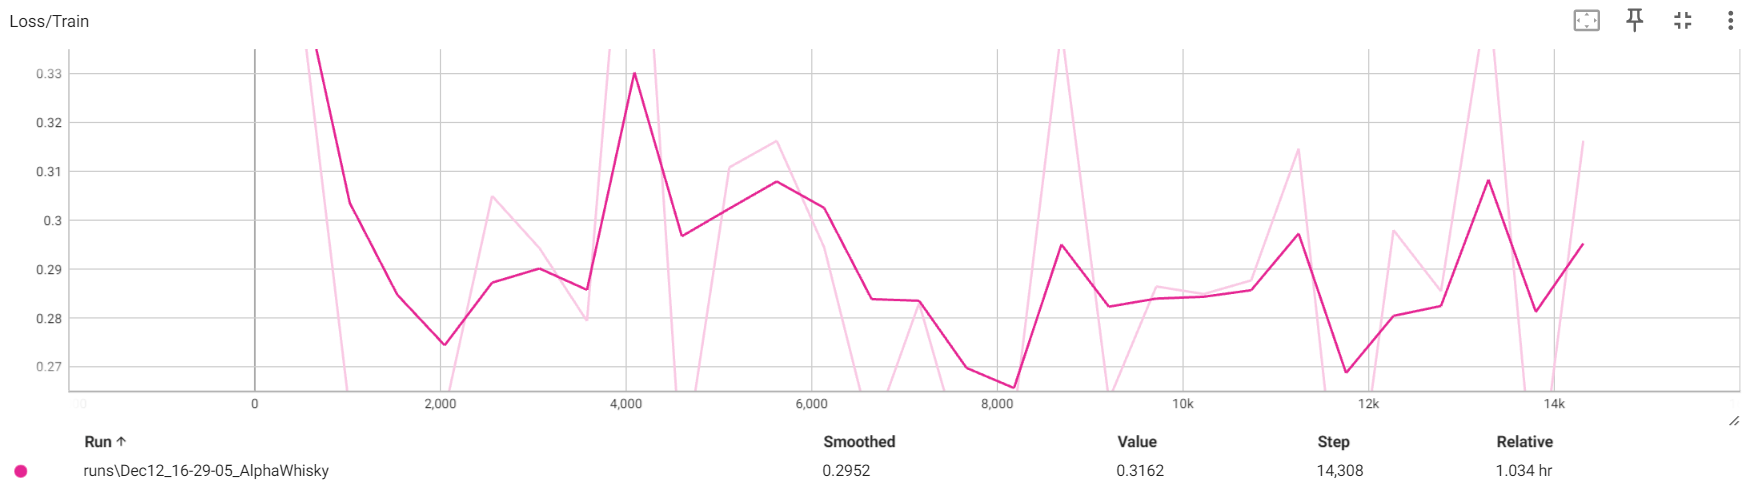
\includegraphics[width=\linewidth]{images/ResNet5_train_loss.jpg}
        \caption{ResNet5 Training Loss}
        \label{fig:train_loss}
    \end{subfigure}%
    \begin{subfigure}{0.5\linewidth}
        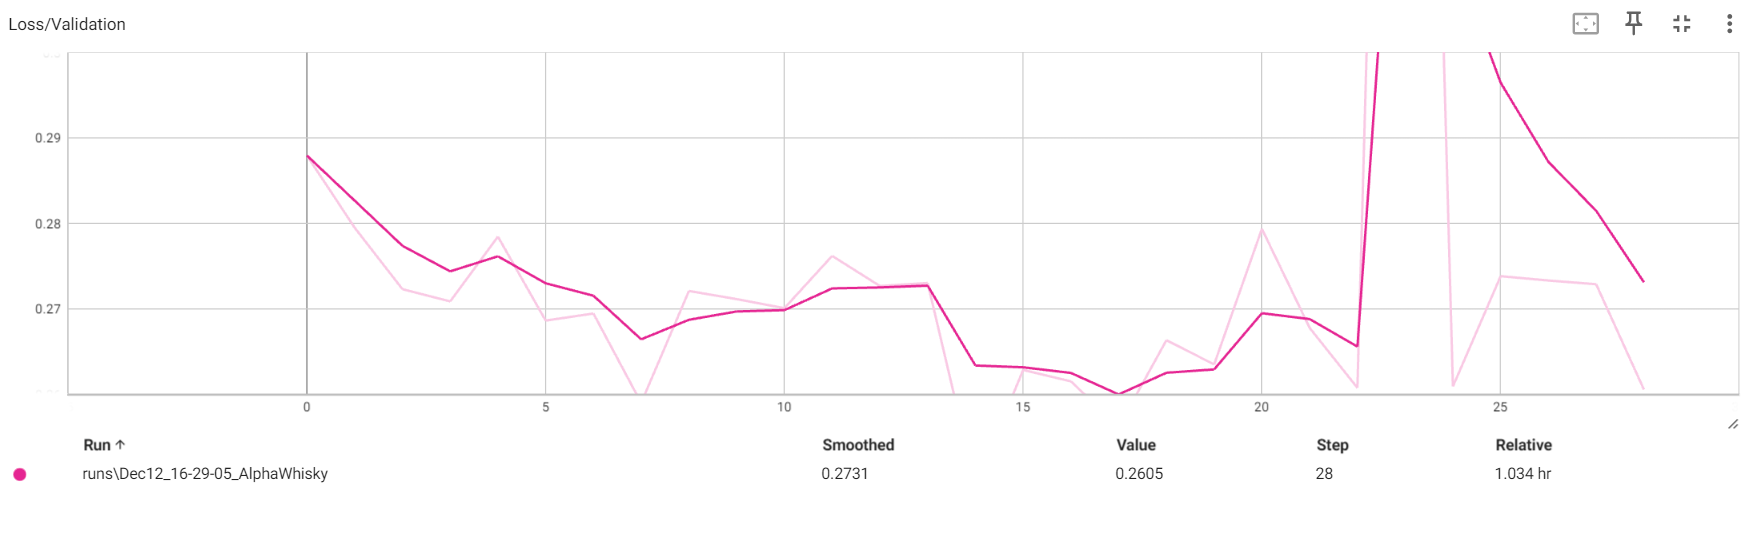
\includegraphics[width=\linewidth]{images/ResNet5_val_loss.jpg}
        \caption{ResNet5 Validation Loss}
        \label{fig:val_loss}
    \end{subfigure}

    \begin{subfigure}{0.5\linewidth}
        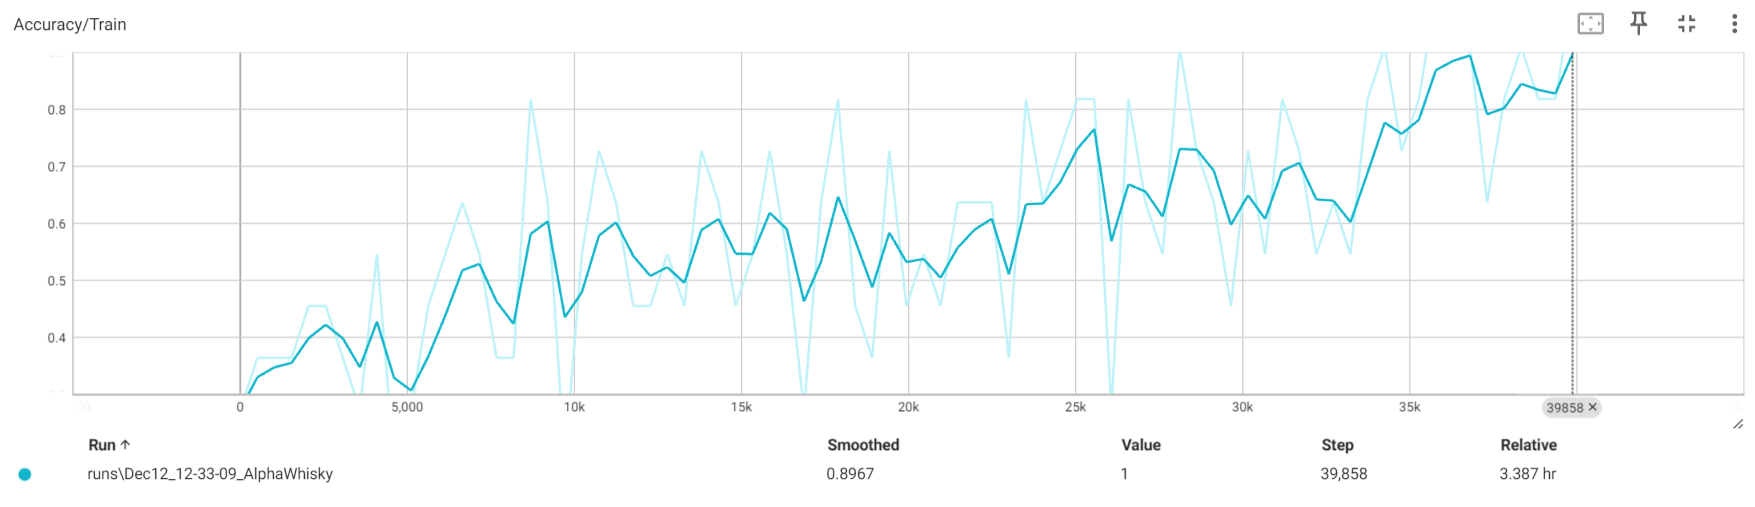
\includegraphics[width=\linewidth]{images/resnet9_train_acc.jpg}
        \caption{ResNet9 Training Accuracy}
        \label{fig:train_acc}
    \end{subfigure}%
    \begin{subfigure}{0.5\linewidth}
        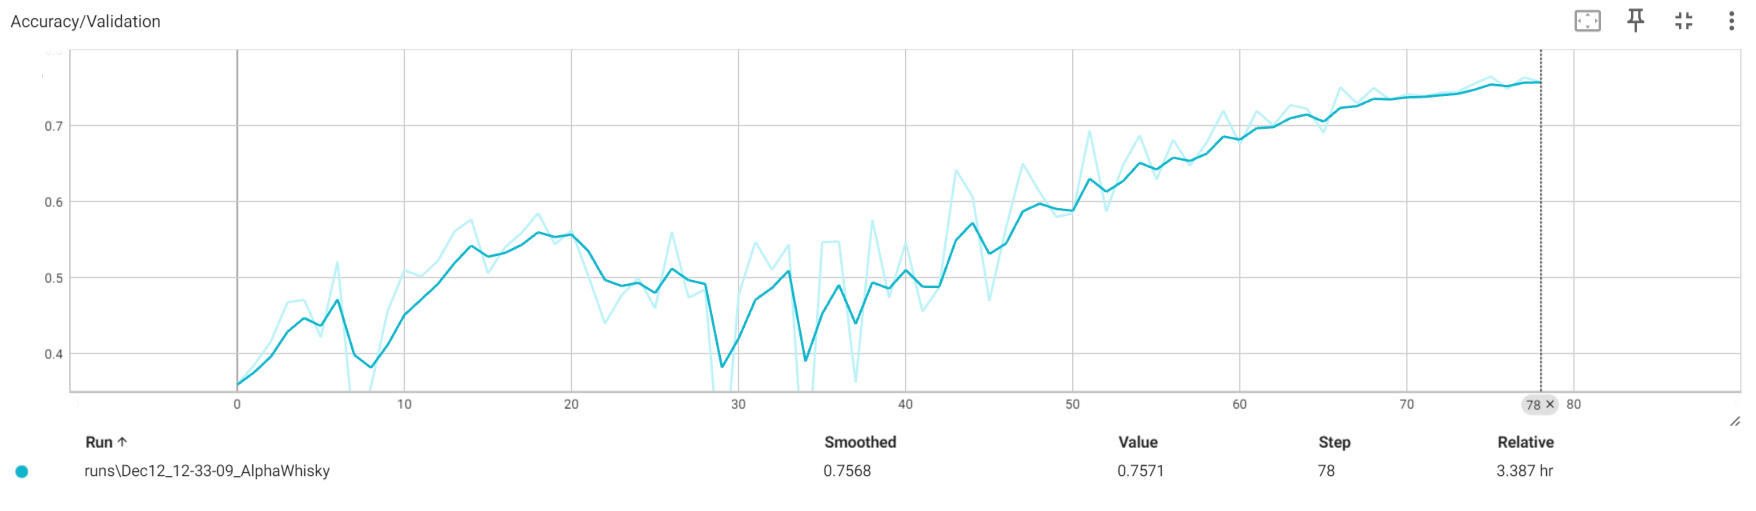
\includegraphics[width=\linewidth]{images/resnet9_val_acc.jpg}
        \caption{ResNet9 Validation Accuracy}
        \label{fig:val_acc}
    \end{subfigure}

    \begin{subfigure}{0.5\linewidth}
        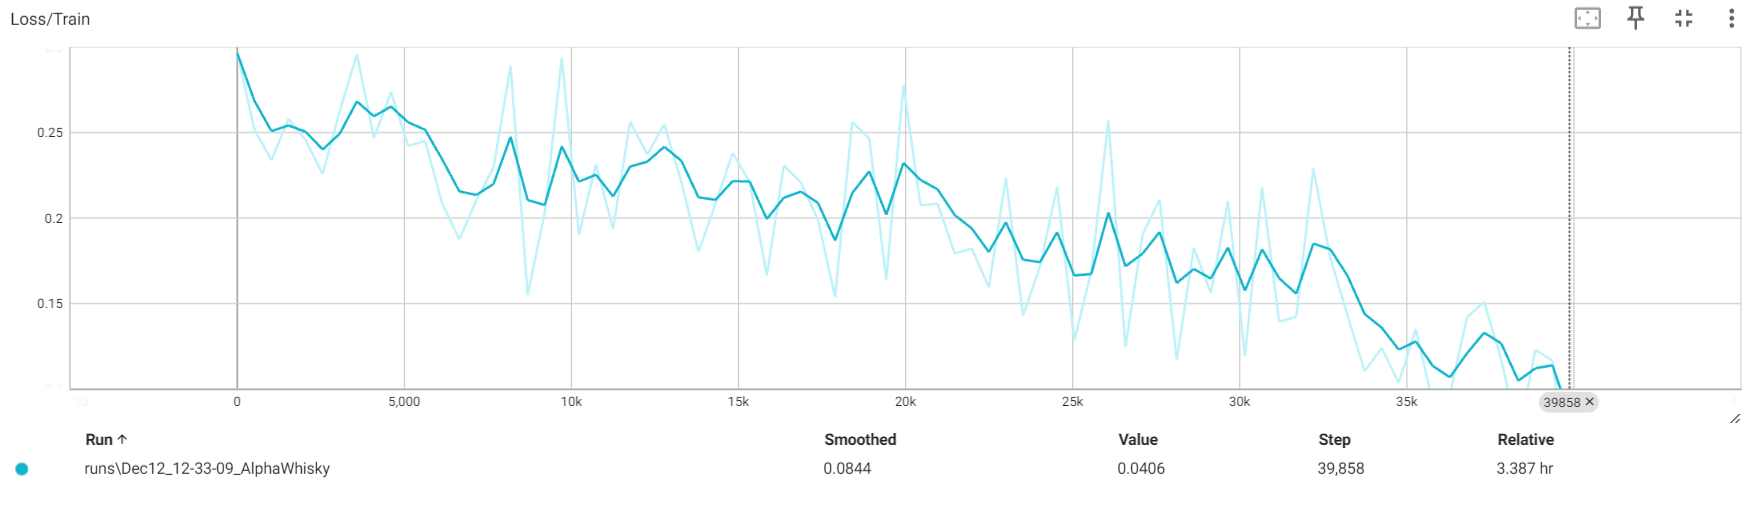
\includegraphics[width=\linewidth]{images/resnet9_train_loss.jpg}
        \caption{ResNet9 Training Loss}
        \label{fig:train_loss}
    \end{subfigure}%
    \begin{subfigure}{0.5\linewidth}
        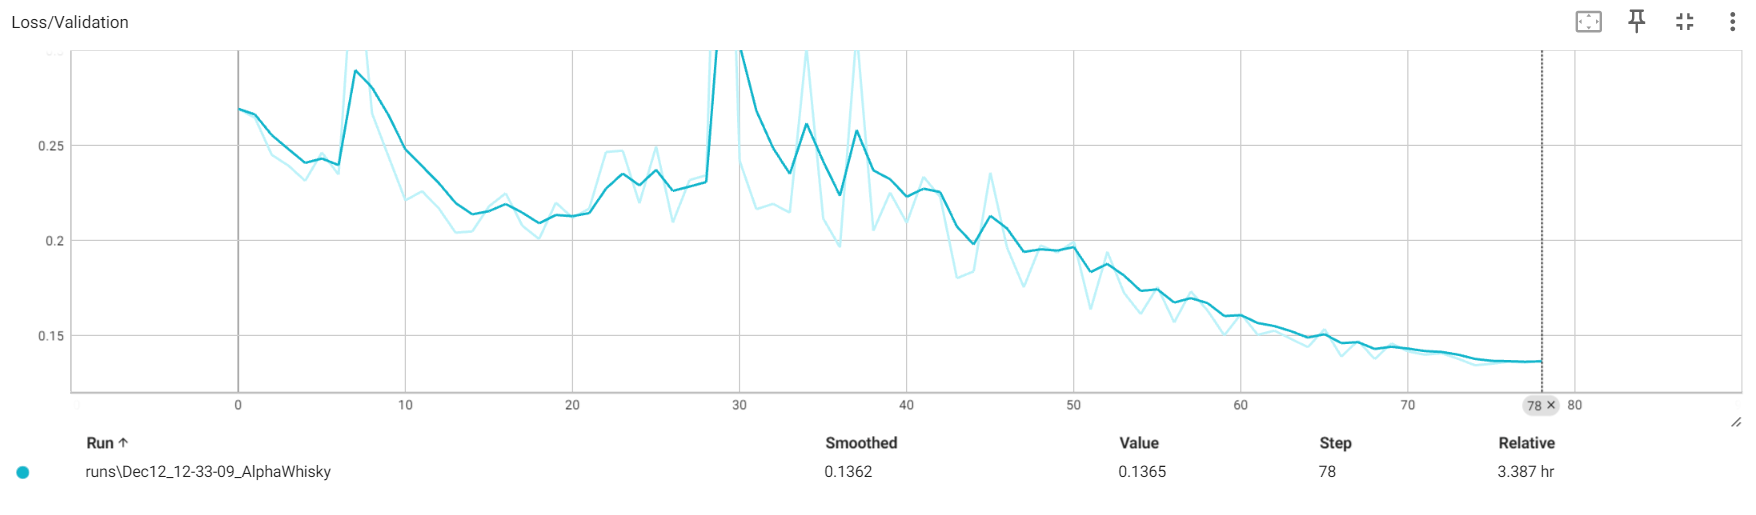
\includegraphics[width=\linewidth]{images/resnet9_val_loss.jpg}
        \caption{ResNet9 Validation Loss}
        \label{fig:val_loss}
    \end{subfigure}

    \caption{ResNet5 and ResNet9 Training and Validation Results}
    \label{fig:resnet_results}
\end{figure}

% The objective of this phase of our research was to construct and refine a Convolutional Neural Network (CNN) model using PyTorch, tailored specifically for the effective classification of various architectural styles. Initially, we embarked on building a custom ResNet 9 model from the ground up. This model was meticulously designed, incorporating a series of stacked residual blocks with convolutional layers, a structure conducive to capturing the intricate details and characteristics of different architectural designs. However, during the initial trials, we encountered the common challenge of overfitting. To address this, we employed several strategic modifications. Firstly, we transitioned to a more simplified model, ResNet 5, effectively reducing the number of layers to decrease the overall complexity of the network. This adjustment helped in mitigating the overfitting issue while maintaining the model's classification efficacy. Additionally, we implemented data augmentation techniques, including rotation, scaling, and horizontal flipping, to enrich our training dataset. This diversity in the training examples further contributed to reducing overfitting by providing the model with a broader range of features to learn from. Lastly, to streamline the model's focus and enhance its accuracy, we simplified the classification categories by consolidating them. This step involved merging similar architectural styles into broader categories, decreasing the categories to classify from 25 to 10, thereby reducing the complexity and potential ambiguity of the classification task. These combined efforts in model construction and refinement significantly contributed to the development of a robust and efficient CNN model for architectural image classification.

\textbf{Build ResNet 9 from scratch}: The objective of this phase of our research was to construct and refine a Convolutional Neural Network (CNN) model using PyTorch, tailored specifically for the effective classification of various architectural styles. We build a ResNet 5 from the ground up to test the baseline performance of the model. According to the performance plots, the ResNet 5 model underfits the dataset and converges quickly. Hence, we build a more expressive model, ResNet 9, to improve the model's training accuracy. However, ResNet 9 turns out to overfit the current dataset.

\textbf{Causes of overfitting}: Normally, a model overfitting a dataset is caused by two conditions -- either the model is too expressive or the dataset is too small. Hence, we come out with two possible approaches to resolving this issue -- regularizing the model or fetching more data. We first apply the data augmentation techniques, including rotation, scaling, and horizontal flipping, to enrich our training dataset. Data augmentation basically enable the model to identify key features from abnormal images, such as images taken in a dark setting or taken from a skewed perspective. The model trained on the augmented dataset performs better than the last version. Then, to streamline the model's focus and enhance its accuracy, we simplified the classification categories by consolidating them. This step involved merging similar architectural styles into broader categories, decreasing the categories to classify from 25 to 10, thereby reducing the complexity and potential ambiguity of the classification task. However, since augmented data share a large portion of key features with the original dataset, the model still reaches a performance bottleneck. Hence, we adopt the regularization technique.

\textbf{Regularization}: We manually add Dropout layers to allow the model to randomly set some fractions of the dataset to 0 at each update and prevent the parameters from co-adapting too much. Compared with its former performance plots, the regularized ResNet9 model produces a higher accuracy in both the training set and the cross-validation set. That is a good sign for the low bias and the low variance.

\textbf{Pivot to transfer learning}: Although we handled the over-fitting issue in the ResNet 9 model, there are two subsequent concerns. Compared with using a pre-trained model, it consumes a significant amount of time and data to train it from scratch. However, it is neither time-efficient nor resource-efficient to train the whole model from the ground up because we can borrow the general image classification capabilities from pre-trained CNN models. Hence, in the next stage, we import a larger pre-trained model and feed our specific dataset.


\subsection{Phase 3: Fine-tuning and Addressing Validation Bottlenecks}

% The objective of this phase was to enhance the model's performance on unseen data, specifically by addressing the noticeable disparity between high training accuracy and comparatively lower cross-validation accuracy. Our methodology began with a meticulous analysis of the model's validation performance. We identified that the high accuracy on training data, juxtaposed with the poor performance on cross-validation data, was a clear indicator of overfitting. To further understand this issue, we plotted learning curves that allowed us to visualize the point of divergence between training and validation accuracy. This analytical approach provided insightful data on how the model learned and where it began to overfit.

In response to prior findings, we pivoted our strategy to include the implementation of transfer learning. This involved utilizing a pre-trained ResNet 18 model, which had been initially trained on a large and diverse dataset, such as ImageNet. The rationale behind this choice was that a model pre-trained on a vast and varied dataset would have already learned a substantial amount of features, which could be beneficial for our task. To tailor this model to our specific needs in architectural image classification, we conducted fine-tuning on the last few layers of the ResNet 18 model. This process involved retraining these layers with our architectural image dataset, allowing the model to adjust its learned features to our specific classification task. This method of integrating transfer learning not only addressed the overfitting issue but also leveraged the advanced learning that the model had already achieved, thus enhancing its performance on new, unseen data.

\subsection{Phase 4: Final Model and Performance Evaluation}

The concluding phase of our project was focused on two key objectives: finalizing the model after iterative refinements and comprehensively evaluating its overall performance. To achieve this, we employed a structured methodology encompassing both the finalization of the model and its subsequent performance assessment.

\textbf{Finalization of the Model:} Our journey of refinement and optimization culminated with the selection of the ResNet 18 model as our final model. This decision was informed by the model's performance during the previous phases, particularly its ability to effectively address the overfitting issues we encountered.

An integral part of this finalization process involved the meticulous optimization of hyper-parameters. Parameters such as learning rate, batch size, and the number of epochs were fine-tuned to align with the performance metrics we aimed to optimize. This step was crucial to ensure that the model not only performed optimally in terms of accuracy but also operated efficiently.

\textbf{Performance Evaluation:} To rigorously assess the model’s performance, we utilized a separate validation set that had not been used during the training phase. This approach was critical to objectively evaluate the model's ability to generalize and perform on new, unseen data.

A suite of metrics was employed to provide a holistic view of the model's performance. These included accuracy, which measures the proportion of correctly predicted instances; precision, indicating the proportion of positive identifications that were actually correct; recall, reflecting the proportion of actual positives that were correctly identified; and the F1 score, which provides a balance between precision and recall. These metrics together offered a comprehensive understanding of the model's strengths and areas for improvement, giving us a detailed picture of its overall effectiveness in classifying architectural styles. In our experiment, the F1 score is 0.93, the recall is 0.93, and the precision is 0.93. These key metrics prove that our model is good enough to identify the correct architecture labels in the picture.

In conclusion, this final phase was pivotal in solidifying the reliability and robustness of our CNN model, ensuring it not only achieved high accuracy but also maintained a balanced performance across various metrics. This rigorous evaluation process was fundamental in affirming the model's readiness for application in real-world scenarios.
\begin{figure}[h]
    \centering

    \begin{subfigure}{0.5\linewidth}
        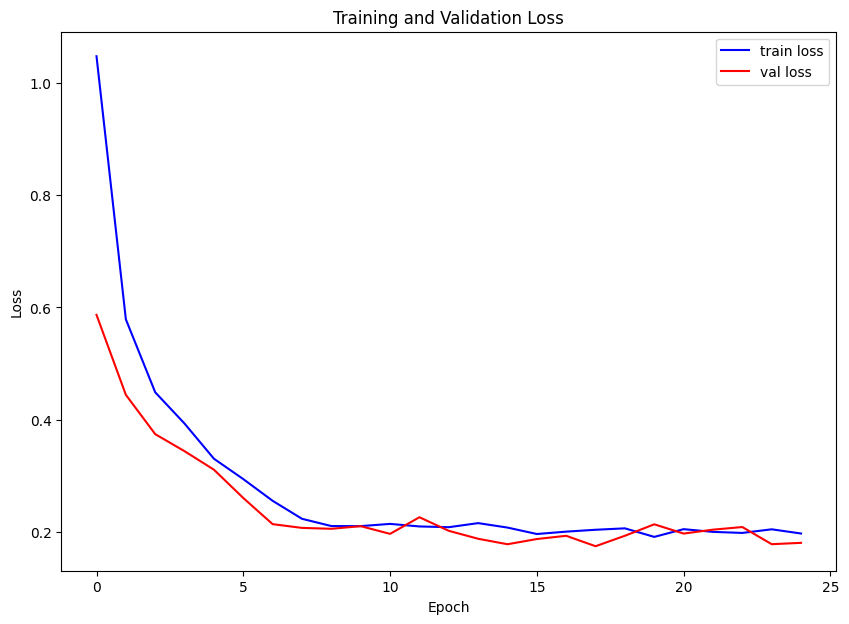
\includegraphics[width=\linewidth]{images/resnet18_loss.png}
        \caption{ResNet18 Training and Validation Loss}
        \label{fig:train_acc}
    \end{subfigure}%
    \begin{subfigure}{0.5\linewidth}
        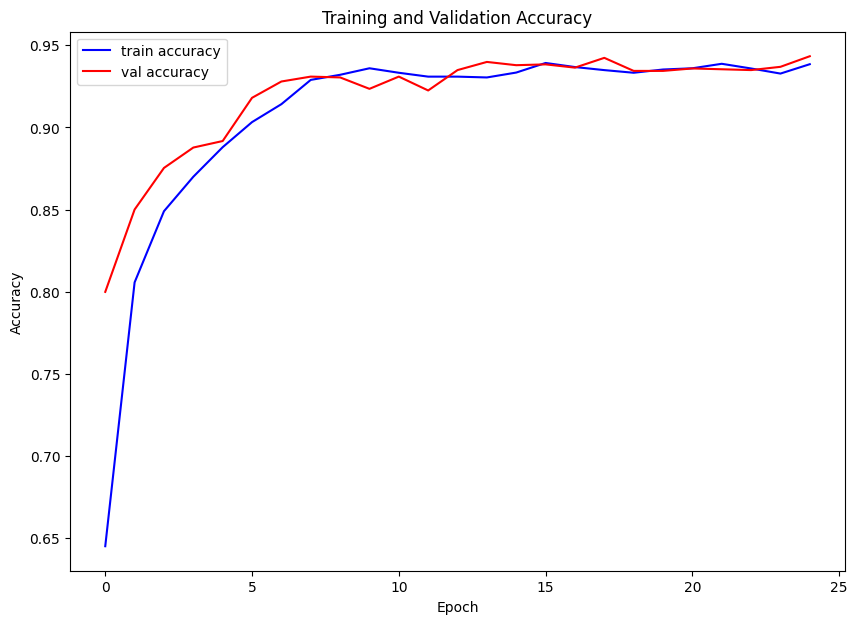
\includegraphics[width=\linewidth]{images/resnet18_accuracy.png}
        \caption{ResNet18 Training and Validation Accuracy}
        \label{fig:val_acc}
    \end{subfigure}

    \caption{ResNet18 Training and Validation Results}
    \label{fig:resnet_results}
\end{figure}

\begin{figure}[h]
    \centering

    \begin{subfigure}{0.5\linewidth}
        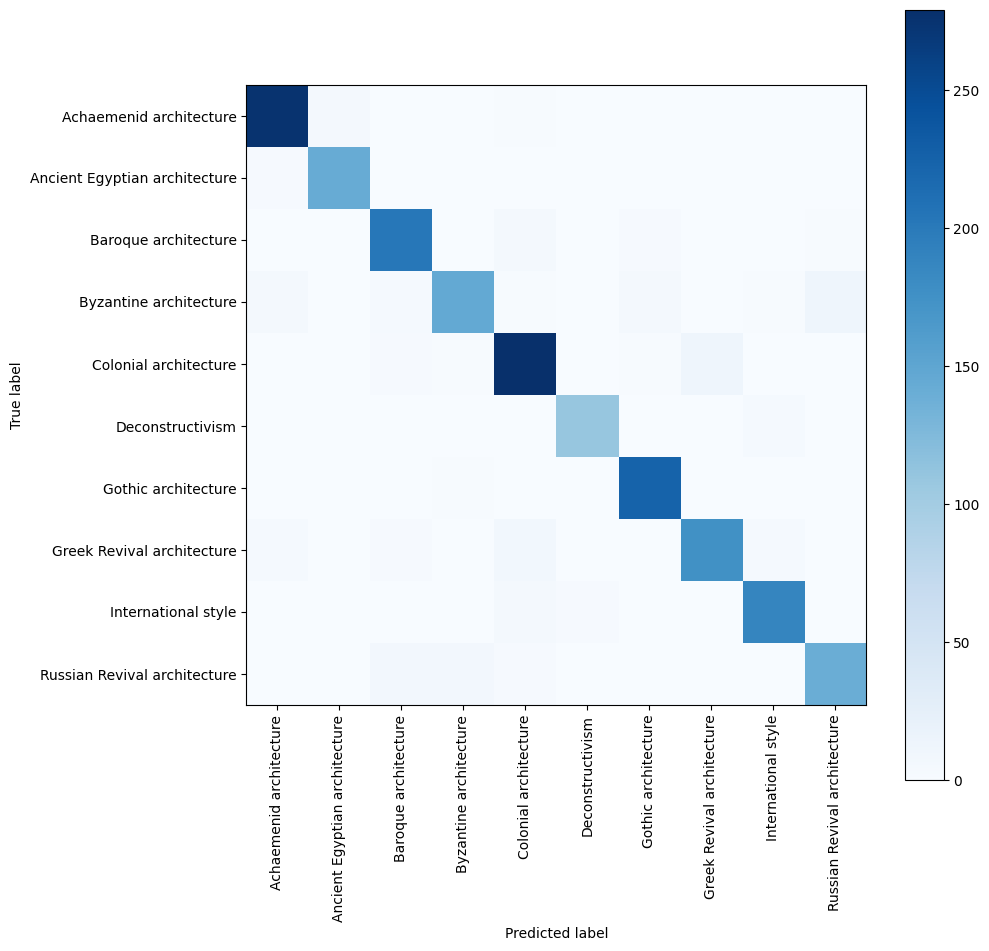
\includegraphics[width=\linewidth]{images/confusion-matrix.jpg}
    \end{subfigure}%

    \caption{ResNet 18 F1-Score Confusion Matrix}
    \label{fig:confusion_matrix}
\end{figure}

\section{Conclusion}

\subsection{Result}

As we conclude this project, it is evident that the development and refinement of the CNN model for architectural image classification has been both challenging and rewarding. The successful implementation of the ResNet 18 model, after navigating through various stages of optimization and problem-solving, demonstrates a significant achievement in the field of computer vision, particularly in the specialized area of architectural style classification. However, like all research endeavors, this project is not without its limitations and avenues for future exploration.

\subsection{Discussion and Future Works}

One of the potential limitations of our current model is the reliance on the dataset used for training and validation. While extensive, there's always room for expanding the dataset to include a wider array of architectural styles, especially those from underrepresented regions or historical periods. Additionally, the current model may face challenges in adapting to drastically different architectural features not present in the training set.

Finally, adapting the model for real-time classification in mobile or web applications could significantly broaden its practical applications, making it a valuable tool for educational purposes, in architectural firms, or for cultural preservation projects.

In summary, the project stands as a testament to the potential of CNNs in specialized image classification tasks, setting a foundation for further research and development in this exciting field of computer vision.

% Here is an example usage of the two main commands (\verb+citet+ and \verb+citep+): Some people thought a thing \citep{kour2014real, hadash2018estimate} but other people thought something else \citep{kour2014fast}. Many people have speculated that if we knew exactly why \citet{kour2014fast} thought this\dots

% \subsection{Figures}
% \lipsum[10]
% See Figure \ref{fig:fig1}. Here is how you add footnotes. \footnote{Sample of the first footnote.}
% \lipsum[11]

% \begin{figure}
% 	\centering
% 	\fbox{\rule[-.5cm]{4cm}{4cm} \rule[-.5cm]{4cm}{0cm}}
% 	\caption{Sample figure caption.}
% 	\label{fig:fig1}
% \end{figure}

% \subsection{Tables}
% See awesome Table~\ref{tab:table}.

% The documentation for \verb+booktabs+ (`Publication quality tables in LaTeX') is available from:
% \begin{center}
% 	\url{https://www.ctan.org/pkg/booktabs}
% \end{center}


% \begin{table}
% 	\caption{Sample table title}
% 	\centering
% 	\begin{tabular}{lll}
% 		\toprule
% 		\multicolumn{2}{c}{Part}                   \\
% 		\cmidrule(r){1-2}
% 		Name     & Description     & Size ($\mu$m) \\
% 		\midrule
% 		Dendrite & Input terminal  & $\sim$100     \\
% 		Axon     & Output terminal & $\sim$10      \\
% 		Soma     & Cell body       & up to $10^6$  \\
% 		\bottomrule
% 	\end{tabular}
% 	\label{tab:table}
% \end{table}

% \subsection{Lists}
% \begin{itemize}
% 	\item Lorem ipsum dolor sit amet
% 	\item consectetur adipiscing elit.
% 	\item Aliquam dignissim blandit est, in dictum tortor gravida eget. In ac rutrum magna.
% \end{itemize}


% \bibliographystyle{unsrtnat}
\bibliography{references}  %%% Uncomment this line and comment out the ``thebibliography'' section below to use the external .bib file (using bibtex) .


%%% Uncomment this section and comment out the \bibliography{references} line above to use inline references.
\begin{thebibliography}{9}

\bibitem{krizhevsky2012imagenet}
A. Krizhevsky, I. Sutskever, and G. E. Hinton, ``ImageNet Classification with Deep Convolutional Neural Networks,'' in \textit{Advances in Neural Information Processing Systems}, 2012, pp. 1097–1105.

\bibitem{shorten2019survey}
C. Shorten and T. M. Khoshgoftaar, ``A survey on Image Data Augmentation for Deep Learning,'' \textit{Journal of Big Data}, vol. 6, no. 1, p. 60, 2019.

\bibitem{szegedy2015going}
C. Szegedy, W. Liu, Y. Jia, P. Sermanet, S. Reed, D. Anguelov, D. Erhan, V. Vanhoucke, and A. Rabinovich, ``Going Deeper with Convolutions,'' in \textit{Proceedings of the IEEE Conference on Computer Vision and Pattern Recognition (CVPR)}, 2015, pp. 1–9.

\bibitem{chollet2017python}
F. Chollet, \textit{Deep Learning with Python}. Manning Publications, 2017.

\bibitem{goodfellow2016deep}
I. Goodfellow, Y. Bengio, A. Courville, and Y. Bengio, \textit{Deep Learning}, vol. 1. MIT press Cambridge, 2016.

\bibitem{yosinski2014transferable}
J. Yosinski, J. Clune, Y. Bengio, and H. Lipson, ``How transferable are features in deep neural networks?,'' in \textit{Advances in Neural Information Processing Systems}, 2014, pp. 3320–3328.

\bibitem{he2016deep}
K. He, X. Zhang, S. Ren, and J. Sun, ``Deep Residual Learning for Image Recognition,'' in \textit{Proceedings of the IEEE Conference on Computer Vision and Pattern Recognition (CVPR)}, 2016, pp. 770–778.


\bibitem{simonyan2014very}
K. Simonyan and A. Zisserman, ``Very Deep Convolutional Networks for Large-Scale Image Recognition,'' \textit{arXiv preprint arXiv:1409.1556}, 2014.

\bibitem{russakovsky2015imagenet}
O. Russakovsky, J. Deng, H. Su, J. Krause, S. Satheesh, S. Ma, Z. Huang, A. Karpathy, A. Khosla, M. Bernstein, A. C. Berg, and L. Fei-Fei, ``ImageNet Large Scale Visual Recognition Challenge,'' \textit{International Journal of Computer Vision}, vol. 115, no. 3, pp. 211–252, 2015.

\bibitem{zhang2018shufflenet}
X. Zhang, X. Zhou, M. Lin, and J. Sun, ``ShuffleNet: An Extremely Efficient Convolutional Neural Network for Mobile Devices,'' in \textit{Proceedings of the IEEE Conference on Computer Vision and Pattern Recognition (CVPR)}, 2018, pp. 6848–6856.

\end{thebibliography}



\end{document}
